\documentclass[journal,12pt,twocolumn]{IEEEtran}
\usepackage{graphicx}
\usepackage{listings}
\usepackage[utf8]{inputenc}
\usepackage{caption}
\usepackage{hyperref}
\usepackage[cmex10]{amsmath}
\usepackage{array}
\usepackage{gensymb}
\usepackage{booktabs}
\usepackage{etoolbox}
\patchcmd{\section}{\centering}{}{}{}
\providecommand{\norm}[1]{\left\lVert#1\right\rVert}
\providecommand{\abs}[1]{\left\vert#1\right\vert}
\let\vec\mathbf
\newcommand{\myvec}[1]{\ensuremath{\begin{pmatrix}#1\end{pmatrix}}}
\newcommand{\mydet}[1]{\ensuremath{\begin{vmatrix}#1\end{vmatrix}}}
\providecommand{\brak}[1]{\ensuremath{\left(#1\right)}}
\makeatletter
\newcommand\xleftrightarrow[2][]{%
  \ext@arrow 9999{\longleftrightarrowfill@}{#1}{#2}}
\newcommand\longleftrightarrowfill@{%
  \arrowfill@\leftarrow\relbar\rightarrow}
\makeatother
\title{Matrix Problems \textbf{\\Straight Lines }}
\author{Manoj Chavva} 

\begin{document}
\maketitle



\section{Problem Statement}

\noindent The base of an equilateral triangle with side 2a lies along the y-axis such that the mid-point of the base is at the origin. Find vertices of the triangle.


\section{Solution}
\noindent Given ABC is an equilateral triangle i.e 
\begin{equation}
AB = BC = CA  
\end{equation}

\begin{figure}[h]
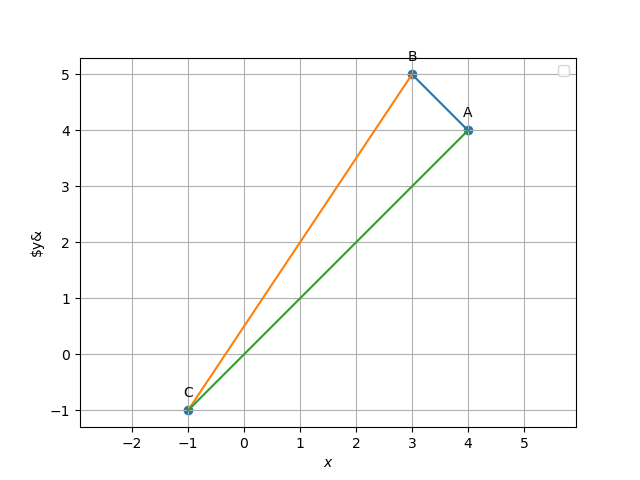
\includegraphics[width=1\columnwidth]{triangle.png}
\caption{Equilateral Triangle ABC}
\label{fig:triangle}
\end{figure}



\noindent Since base with 2a is lies on the y-axis with the mid-point of the base is at origin. The vertices of the two points on y-axis will be

\begin{equation}
\vec{B}=\begin{pmatrix} 
0\\
a
\end{pmatrix}, {
\vec{C}=\begin{pmatrix} 
0\\
-a
\end{pmatrix} }
\end{equation}
%$\vec{B}(0 , a)$ and $\vec{A}(x, y)$ 

%\noindent It is known that the line joining a vertex of an equilateral triangle with the midpoint of its opposite side is perpendicular. \\


%\noindent Since, the mid point lies on origin. The vertex \textbf{A} lies on the x-axis.\\

%\noindent So, The vertex will be \\


%begin{equation}
%\vec{A}=\begin{pmatrix} 
%x\\
%0
%\end{pmatrix}
%\end{equation}

\noindent The distance between the two points B and A is
%\begin{equation}
%\vec{B} = \myvec{0 \\ a}, \vec{A}=\myvec{x \\ 0}
%\end{equation}

\begin{equation}	
\vec{B}-\vec{A} = \myvec{0-x \\ a-y}
\end{equation}

\noindent Using the definition   of the norm, 
		\begin{equation}
\norm{\vec{B}-\vec{A}} =\norm{\myvec{-x \\ a-y}}
\end{equation}
\noindent Since, the side of an equilateral triangle is 2a	
\begin{equation}						
			2a=\sqrt{\myvec{-x & a-y}\myvec{-x \\ a-y}} 
\\
\end{equation}
\begin{equation}						
2a =  \sqrt{(x)^2+ (a-y)^2}
\end{equation}
\texttt\noindent Squaring on both sides

\begin{equation}						
4a^2 =  {(x)^2+ (a-y)^2}
\end{equation}
\begin{equation}
4a^2 = {x^2 + a^2 +y^2-2ay}
\end{equation}
\begin{equation}
3a^2 = {x^2+y^2-2ay}
\label{eq-1-}
\end{equation}

\noindent Similarly, The distance between the two points C and A is

\begin{equation}	
\vec{C}-\vec{A} = \myvec{0-x \\ -a-y}
\end{equation}

\noindent Using the definition   of the norm, 
		\begin{equation}
\norm{\vec{C}-\vec{A}} =\norm{\myvec{-x \\ -a-y}}
\end{equation}
\noindent Since, the side of an equilateral triangle is 2a	
\begin{equation}						
			2a=\sqrt{\myvec{-x & -a-y}\myvec{-x \\ -a-y}} 
\end{equation}
\begin{equation}						
2a =  \sqrt{(x)^2+ (a+y)^2}
\end{equation}
%\texttt{•}
\noindent Squaring on both sides
\begin{equation}						
4a^2 =  {(x)^2+ (a+y)^2}
\end{equation}
\begin{equation}
4a^2 = {x^2 + a^2 +y^2+2ay}
\end{equation}
\begin{equation}
3a^2 = {x^2+y^2+2ay}
\label{eq-2-}
\end{equation}
%\begin{equation}
%\vec{AX} = \vec{B}
%\end{equation}
%Solving equation  and , we get


Using equation (\ref{eq-1-}) and (\ref{eq-2-}),
%\begin{equation}
%  \begin{pmatrix}
%1 & 2a & 1\\
%1 & -2a & 1
%\end{pmatrix} 
%\begin{pmatrix}
%x^2\\
%y\\
%y^2
%\end{pmatrix} 
%=
%\begin{pmatrix}
%3a^2 \\ 
%3a^2\
%\end{pmatrix}
%\end{equation} 

%
%The augmented matrix for the above matrix equation is 
%\vspace{3mm}
%\begin{equation}
%\begin{pmatrix}
% 1 & 2a & 1 & \vrule & 3a^2\\
% 1 & -2a & 1  &\vrule & 3a^2
%    \end{pmatrix}  
%    \end{equation}
%    \begin{center}
%   $\xleftrightarrow{\text{$R_2$ $\leftarrow  {R_2}-{R_1}$}}$
%$ \begin{pmatrix}
%  1 & 2a & 1 &\vrule & 3a^2\\
% 0 & -4a & 0  &\vrule & 0	  
%  \end{pmatrix}$ \\
%   \end{center}
%   \begin{center}
%$ \xleftrightarrow{\text{$R_2$ $\leftarrow  \frac{R_2}{{-4a}} $}} $
%$\begin{pmatrix}
% 1 & 2a & 1 & \vrule & 3a^2\\
%  0 & 1 & 0 &\vrule & 0\
%  \end{pmatrix}$
%  \\
%  \end{center}
%  \begin{center}
%  $ \xleftrightarrow{\text{$R_1$ $\leftarrow  {R_1}-{2aR_2}$}} $
%$\begin{pmatrix}
%  1 & 0 & 1 & \vrule & 3a^2\\
%  0 & 1 & 0 &\vrule & 0\
%  \end{pmatrix}$
%  \\
%  \end{center}
%  \begin{equation}
%\implies X = 
%   \begin{pmatrix}
%   3a^2 \\ 0
%   \label{eq-3-}
% \end{pmatrix}
% \end{equation}
%Using equation (\ref{eq-3-}) we get ,
%\begin{equation}
%	y = 0 \vspace{2mm}
%\end{equation}
%\begin{equation}
%	x^2 = 3a^2 
%\end{equation}
%\begin{equation}						
%x =  \pm\sqrt{3}a 
%\end{equation}
%\begin{equation}						
%y=0
%\end{equation}


\noindent Hence,the coordinates of the vertices of triangle are 
%\begin{equation*}						
%\vec{A} = (\pm\sqrt{3}a,0)\\
%\end{equation*}
%\begin{equation*}						
%\vec{B} = (0,a)\\
%\end{equation*}
%\begin{equation*}						
%\vec{C} = (0,-a)\\
%\end{equation*}

  \begin{equation*}
\vec{A} = 
   \begin{pmatrix}
   \pm\sqrt{3}a \\ 0
 \end{pmatrix}
 \end{equation*}

\begin{equation}
\vec{B}=\begin{pmatrix} 
0\\
a
\end{pmatrix}, {
\vec{C}=\begin{pmatrix} 
0\\
-a
\end{pmatrix} }
\end{equation}

\newpage
\section{Construction}
B and C are the inputs.
\begin{table}[h]
\centering
\large
\begin{tabular}{|l|l|l|}
\hline
\textbf{Symbol} & \textbf{Value} & \textbf{Description} \\ \hline
B               & (0, 2)         & Vertex B             \\ \hline
C               & (0, -2)        & Vertex C             \\ \hline
A               & (x,y)          & Vertex A             \\ \hline
A1              & (x1, y1)       & Vertex A1            \\ \hline
\end{tabular}
\end{table}

\begin{table}[h]
\large
\begin{tabular}{lll}
\multicolumn{3}{l}{Get Python Code for image from}                                                 \\ \hline
\multicolumn{3}{|l|}{\url{https://github.com/ManojChavva/FWC/blob/main/Matrix/line/code-py/triangle.py}} \\ 
 \hline
%\multicolumn{3}{l}{Get LaTex code from}                                                            \\ \hline
%\multicolumn{3}{|l|}{\url{https://github.com/ManojChavva/FWC/blob/main/Matrix/line/line.tex}}            \\ \hline
\end{tabular}
\end{table}

\end{document}
